\subsection{Individual Monitor}
\subsubsection{Problem Definition}
The individual circuit monitors provide the means for the homeowner to know where power is used within the building and makes up the second half of the smart breakers, along with the switching circuitry. They measure voltage and current in the connected home circuit, use it for controlling the breakers and feed the information to the user through the base station. Homeowners can then use the information to adjust their power consumption habits, while the control logic uses the information to detect over-current and over-voltage situations and change the switch's status accordingly. 

\subsubsection{System Diagram}
\begin{figure}[htbp]
\begin{center}
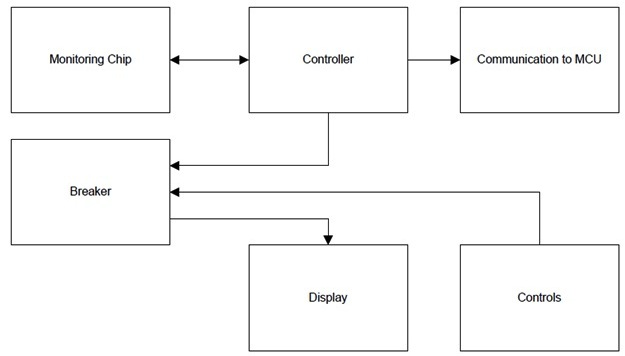
\includegraphics[width=5in]{includes/NJMonitorSystemDiagram}
\caption{Block diagram of monitioring system}
\label{fig:monitor_system_diagram}
\end{center}
\end{figure}

The above diagram shows the components of the individual monitors and their relationships to each other and the breaker section of the smart breakers. 

\subsubsection{System Components}
%Metering Chip
The purpose of the metering chip and its inputs is to measure instantaneous voltage and current and pass the data to the controller. 

At the beginning of the year, the team found ADE7763 metering chips from Analog Devices and obtained free samples. As an IC designed for energy metering [ADE datasheet], the chip has all of the functionality needed for the project. At a minimum, the chip needs to read voltage and current with additional measurements being nice but not necessary. The team also found several other chips that perform similarly, but due to cost, the team decided to use the ADE7763 metering chips. 

Input methods for the ADE7763 were selected based on the AN 564 app note, using a current transformer and voltage divider to measure the power line. Both work well for the project because they are simple and accurate. The current transformer is more expensive than the team hoped, but was easily available and the voltage divider is both easily available and low cost. Selected components and values keep the input levels lower than the maximum value of $500 \mV$ %[ADE datasheet citation] 
for the ADE7763 channels using the equations below.

%insert CT voltage equation here
\begin{equation}
V_{secondary}=\frac{(I_{primary}\times R_{burden})}{2511}
\end{equation}

This gives the voltage across the secondary of the current transformer and comes from the datasheet for the current transformer %[CT datasheet citation]. 
From this equation, $R_{burden}$ is selected as $60 \ohm$, allowing the current transformer to be used for up to $20\ampere$.

%insert voltage divider and power equations here
\begin{equation}
V_{measure}=V_{line}\times \frac{R_{measure}}{R_{total}}
\end{equation}

\begin{equation}
P=\frac{V^2}{R}
\end{equation}

The first equation is the standard voltage divider equation used to determine values so the maximum input voltage is not exceeded. The second equation is the power equation used to determine resistor values so they don't burn up. To keep $V_{measure}$ under $500\milli \V$, $R_{measure}$ is $1\kilo\ohm$ with an $R_{total}$ of $511\kilo\ohm$. 

%insert cutoff frequency equation here
\begin{equation}
f_{3dB}=\frac{1}{2\pi(R)(C)}
\end{equation}

This equation is used to determine the 3dB point of the attenuation network in Figure \ref{fig:attenuation_network} \cite{AN564}. A $22\nano\farad$ capacitor with the $R_{measure}$ from above gives a cutoff of $7200\hertz$ as suggested by the app note \cite{AN564}. 

\begin{figure}[htbp]
\begin{center}
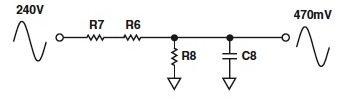
\includegraphics[width=3in]{includes/NJAttenuationNetwork} 
\caption{Attenuation network for ADE7763 \cite{AN564}.}
\label{fig:attenuation_network} 
\end{center}
\end{figure}

%Microcontroller
The microcontroller's job is to transfer the data stored in the metering chip's registers to the base station and does so through the SPI connection to the chip that's provided. It also provides the logic needed to detect and turn off the breaker in an over-voltage or over-current.  Other functions include managing start up and shut down, primarily initializing registers and saving data. 

First semester, the team decided to use an FPGA for this purpose as they are very flexible and can easily manage data from the metering chip. However, the design process for the rest of the breakers took longer than anticipated and the team decided to use the Altera Nios II processor available from Calvin. Calvin also had some pic microcontrollers, but the team is not familiar with them and would have had to learn new protocols and language, making the design more complex than the Nios II which had been used in other classes before. After working with the Nios II, the team discovered there is very little documentation for the function needed, making it very difficult to work with. The team decided to look at possible alternatives and found an Arduino Uno that uses an ATmega328 microcontroller and has more and clearer documentation. 

\begin{figure}[htbp]
\begin{center}
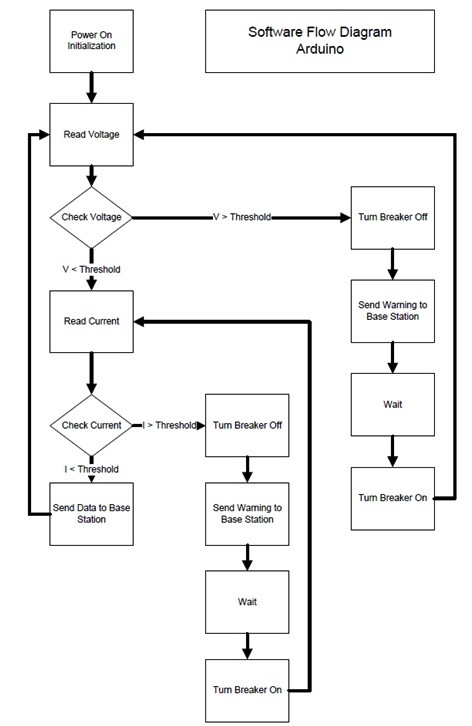
\includegraphics[width=5in]{includes/NJArduinoSoftwareFlow}
\caption{Software flow diagram for Arduino microcontroller}
\label{fig:arduino_software_flow}
\end{center}
\end{figure}

\begin{figure}[htbp]
\begin{center}
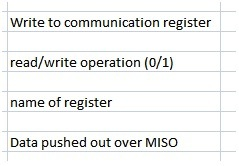
\includegraphics[width=3in]{includes/NJADEread} 
\caption{Read/write process for ADE7763}
\label{fig:ade_read}   
\end{center}
\end{figure}

Figure \ref{fig:arduino_software_flow} shows the microcontroller's operating process for normal operation and what it does in both an over\-voltage and over\-current situation. Voltage and current are both necessary to calculate power, so the team focused on reading those values first. Other features of the ADE7763 may be used if the project were given more time, but as they're not critical, the team didn't deal with them since the ADE7763 makes it easy to ignore information it collects. 

Figure \ref{fig:ade_read} is an expanded view of the read operation in Figure \ref{fig:arduino_software_flow} and includes the write process in addition to the read process for communicating with the ADE7763.

%Communication
The purpose of the communication component is to transfer data from the smart breakers to the base station and is controlled by the microcontroller. 

First semester the team decided to use Ethernet to achieve this, based on compatibility with the base station, low cost and ability to connect several breakers. However, longer than expected design time for other aspects of the project made it necessary to use a simpler method. The team chose XBee radios instead, which use RS232 to connect, lowering the design time. XBee also removes the need to have external wires connecting the breakers and base station, making the product more aesthetically appealing to the customer. 

%Display
The purpose of the display is to provide the user with basic on/off information relating to the breakers should the system fail and require a manual shutoff. This meant it must be simple and easy to understand, which led to the decision to use well-labeled LEDs. Because LEDs are very easy to include in a schematic, using them instead of a character-based display also reduced design time.  

%Controls
Because it can be critical to shut off power, the team decided to include a physical failsafe method in addition to the system's ability to do so automatically. Because of the way the automatic switching is configured, this backup switch would only allow the user to turn power off \- they will not be able to override the controls and force an over-voltage or over-current situation.

\subsubsection{Final Decisions}
To summarize, the individual circuit monitors consist of an Arduino Uno microcontroller and Analog Devices ADE7763 metering chip with input networks using a voltage divider and current transformer. The unit will communicate with the base station computer through the Arduino to computer interface directly, using SPI for communication between the ADE7763 and Arduino Uno. Minimal on/off displays and controls including LEDs and a physical switch will be provided to ensure user safety as well. The system will use a solid state relay to demonstrate that the microcontroller is able to control a switching device, but will use a yet to be determined technology for a marketable product.

\subsubsection{Printed Circuit Board}
%to be completed later

\subsubsection{Testing}
%Inputs to ADE7763
The table and graph below show the results of current transformer testing. During testing, a $6.2\kilo\ohm$ burden resistor was used instead of the $60 \ohm$ selected for final design to make it easier to read results using an oscilloscope. Table 1 gives the component values used and the resulting voltage and current measurements, both with percent error from values calculated based on measurements on the primary side. 

\begin{table}[htdp]
\caption{Measured:Primary}
\begin{center}
\begin{tabular}{|c|c|c|c|c|} \hline
Desc. & Voltage($\volt$) & Power ($\watt$) & Resistance ($\ohm$) & Current ($\ampere$) \\ \hline
1 S & 117 & 40.00 & 342 & 0.360 \\ \hline
2 S & 117 & 20.00 & 684 & 0.250 \\ \hline
3 S & 117 & 13.33 & 1027 & 0.210 \\ \hline
4 S & 117 & 10.00 & 1369 & 0.200 \\ \hline
2 Prll & 117 & 80.00 & 171 & 0.690 \\ \hline
\end{tabular}
\end{center}
\label{tab:measured_primary}
\end{table}%

\begin{table}[htdp]
\caption{Measured:Secondary with Percent Error}
\begin{center}
\begin{tabular}{|c|c|c|c|c|c|} \hline
Desc. & Voltage($\volt$) & \% Error & Resistance ($\ohm$) & Current ($\milli\ampere$) & \% Error \\ \hline
1 S & 0.840 & 5.5 & 6200 & 0.135 & 5.8 \\ \hline
2 S & 0.580 & 6.0 & 6200 & 0.093 & 6.6 \\ \hline
3 S & 0.490 & 5.5 & 6200 & 0.084 & 0.4 \\ \hline
4 S & 0.440 & 10.9 &6200 & 0.069 & 13.4 \\ \hline
2 Prll & 1.620 & 4.9 & 6200 & 0.265 & 3.6 \\ \hline
\end{tabular}
\end{center}
\label{tab:measured_secondaryPercentError}
\end{table}%

\begin{figure}[htbp]
\begin{center}
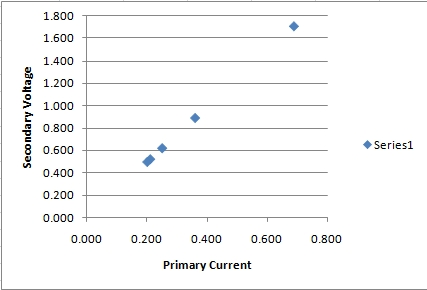
\includegraphics[width=4in]{includes/NJGraph}
\caption{Current-Voltage Response of Current Transformers}
\label{fig:current_transformers_iv_response}
\end{center}
\end{figure}

\begin{figure}[htbp]
\begin{center}
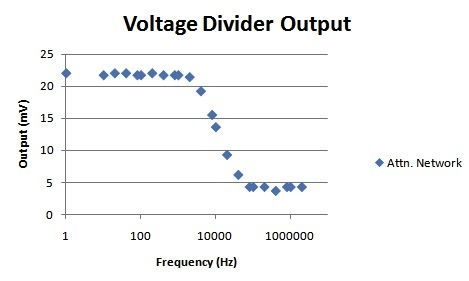
\includegraphics[width=4in]{includes/NJVoltDivOutput}
\caption{Graph showing results from voltage divider testing}
\label{fig:voltage_divider_testing}
\end{center}
\end{figure}

